% Graphic for TeX using PGF
% Title: /home/enberg/Documents/Thesis/assets/uml/Diagram3.dia
% Creator: Dia v0.97.2
% CreationDate: Mon Apr 28 21:27:22 2014
% For: enberg
% \usepackage{tikz}
% The following commands are not supported in PSTricks at present
% We define them conditionally, so when they are implemented,
% this pgf file will use them.
\ifx\du\undefined
  \newlength{\du}
\fi
\setlength{\du}{15\unitlength}
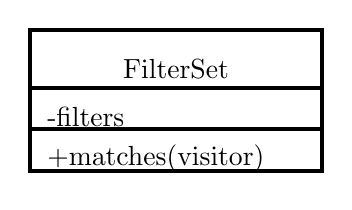
\begin{tikzpicture}
\pgftransformxscale{1.000000}
\pgftransformyscale{-1.000000}
\definecolor{dialinecolor}{rgb}{0.000000, 0.000000, 0.000000}
\pgfsetstrokecolor{dialinecolor}
\definecolor{dialinecolor}{rgb}{1.000000, 1.000000, 1.000000}
\pgfsetfillcolor{dialinecolor}
\pgfsetlinewidth{0.100000\du}
\pgfsetdash{}{0pt}
\definecolor{dialinecolor}{rgb}{1.000000, 1.000000, 1.000000}
\pgfsetfillcolor{dialinecolor}
\fill (11.850000\du,9.700000\du)--(11.850000\du,11.100000\du)--(18.895000\du,11.100000\du)--(18.895000\du,9.700000\du)--cycle;
\definecolor{dialinecolor}{rgb}{0.000000, 0.000000, 0.000000}
\pgfsetstrokecolor{dialinecolor}
\draw (11.850000\du,9.700000\du)--(11.850000\du,11.100000\du)--(18.895000\du,11.100000\du)--(18.895000\du,9.700000\du)--cycle;
% setfont left to latex
\definecolor{dialinecolor}{rgb}{0.000000, 0.000000, 0.000000}
\pgfsetstrokecolor{dialinecolor}
\node at (15.372500\du,10.650000\du){FilterSet};
\definecolor{dialinecolor}{rgb}{1.000000, 1.000000, 1.000000}
\pgfsetfillcolor{dialinecolor}
\fill (11.850000\du,11.100000\du)--(11.850000\du,12.100000\du)--(18.895000\du,12.100000\du)--(18.895000\du,11.100000\du)--cycle;
\definecolor{dialinecolor}{rgb}{0.000000, 0.000000, 0.000000}
\pgfsetstrokecolor{dialinecolor}
\draw (11.850000\du,11.100000\du)--(11.850000\du,12.100000\du)--(18.895000\du,12.100000\du)--(18.895000\du,11.100000\du)--cycle;
% setfont left to latex
\definecolor{dialinecolor}{rgb}{0.000000, 0.000000, 0.000000}
\pgfsetstrokecolor{dialinecolor}
\node[anchor=west] at (12.000000\du,11.800000\du){-filters};
\definecolor{dialinecolor}{rgb}{1.000000, 1.000000, 1.000000}
\pgfsetfillcolor{dialinecolor}
\fill (11.850000\du,12.100000\du)--(11.850000\du,13.100000\du)--(18.895000\du,13.100000\du)--(18.895000\du,12.100000\du)--cycle;
\definecolor{dialinecolor}{rgb}{0.000000, 0.000000, 0.000000}
\pgfsetstrokecolor{dialinecolor}
\draw (11.850000\du,12.100000\du)--(11.850000\du,13.100000\du)--(18.895000\du,13.100000\du)--(18.895000\du,12.100000\du)--cycle;
% setfont left to latex
\definecolor{dialinecolor}{rgb}{0.000000, 0.000000, 0.000000}
\pgfsetstrokecolor{dialinecolor}
\node[anchor=west] at (12.000000\du,12.800000\du){+matches(visitor)};
\end{tikzpicture}
